\documentclass{article}
\usepackage{amsmath}

\usepackage{full page}  % make the margins somewhat smaller than the default

\usepackage{listings}  %  needed for source code listings
\usepackage{color}
\usepackage{hyperref}
\usepackage{graphicx}
%\usepackage[tight,footnotesize]{subfigure}
\usepackage{caption}
\usepackage{subcaption}

\graphicspath{ {Images/} }

\definecolor{javared}{rgb}{0.7,0,0} % for strings
\definecolor{javagreen}{rgb}{0.25,0.6,0.35} % comments
\definecolor{javapurple}{rgb}{0.55,0,0.40} % keywords
\definecolor{javadocblue}{rgb}{0.25,0.35,0.85} % javadoc
 
\lstset{language=Java,
basicstyle=\ttfamily,
keywordstyle=\color{javapurple}\bfseries,
stringstyle=\color{javared},
commentstyle=\color{javagreen},
morecomment=[s][\color{javadocblue}]{/**}{*/},
numbers=left,
numberstyle=\tiny\color{black},
stepnumber=2,
numbersep=10pt,
tabsize=2,
showspaces=false,
showstringspaces=false,
frame=shadowbox,
numbers=left
} 

% set the document title, author, and date here.
%  once set, the \maketitle command (within the document)
%  will display them nicely
\title{AI Assignment 3 - Motion Planning}
\author{Tianyuan Zhang}

\begin{document}
\maketitle

\section{Introduction}
Motion planning is a very important topic in Artificial Intelligence Field. It is obvious that in a coordination the possible next step would be infinite and we cannot simulate an "infinite" thing in the computer world. In this assignment, we will try to solve the motion planning problem by transform this problem into a finite state problem, by using PRM(Probabilistic RoadMap) and RRT(Rapid Exploring Random Tree).

\section{Probabilistic RoadMap}
\subsection{Basic Idea}
The basic idea of PRM is simple. The first step is to sample a number of nodes in configuration space and construct a graph under some kind of constraint. The the second step is to use a normal graph search method to find a path from the start node to the goal node, and we find the motion plan.

More specifically, for this problem, as we are dealing with an arms system, the configuration for each node in the configuration space is the series of angle for their corresponding link. In the sampling stage, we random sample N configuration points. Then for each node we find its k nearest nodes and link the k nodes as the children. Then a normal A* search is applied and if there is a path from the starting node to the goal node, we are done. Otherwise, either such motion is impossible, or our amount of sampling is not enough.

\subsection{Code Implementation}
\subsubsection{constructor}
The constructor sets the starting node, goal node, world, density and the neighbour number k. Then it calles the method $sampling(long) : void$ and $constructMap() : void$ to construct the map.
\begin{lstlisting}
	public ArmProblem(int num, double[] s, double[] g, double[] b, 
			World w, int k, int d, double sr, long seed) {
		base = new double[2];
		base[0] = b[0];
		base[1] = b[1];
		width = 10;
		link_num = num;
		// set start and goal configuration
		start_config = new double[link_num];
		for (int i = 0; i < link_num; i++)
			start_config[i] = s[i];
		goal_config = new double[link_num];
		for (int i = 0; i < link_num; i++)
			goal_config[i] = g[i];
		// set link length
		link_len = new double[link_num];
		for (int i = 0; i < link_num; i++)
			link_len[i] = 30;
		world = w;
		k_neigh = k;
		samples = new HashSet<ArmProblemNode>();
		adjList = new HashMap<>();
		density = d;
		startNode = new ArmProblemNode(start_config, 0, this);
		step_ratio = sr;

		sampling(seed);
		System.out.println("Sampling Done");
		System.out.println("Constructing Map...");
		constructMap();
	}
\end{lstlisting}

\subsubsection{sampling}
The method $sampling():void$ simply generate $density$ number of sample nodes. Nodes must not collide with any of the obastacles in the world.
\begin{lstlisting}
	// sampling the points in configuration space
	public void sampling(long seed) {
		Random rd = new Random(seed);
		samples.add(new ArmProblemNode(start_config, this));
		samples.add(new ArmProblemNode(goal_config, this));
		double[] randConfig = new double[link_num];
		while (samples.size() < density + 2) {
			for (int i = 0; i < link_num; i++)
				randConfig[i] = Math.PI * 2 * rd.nextDouble();
			ArmProblemNode cur = new ArmProblemNode(randConfig, this);
			if (!cur.armCollision(world) && !samples.contains(cur))
				samples.add(cur);
		}
	}
\end{lstlisting}

\subsubsection{constructMap}
In the method $constructMap():void$, for each sample node, k nearest neightbour nodes will be found and linked. A adjacent table will be generated after the map is constructed.
\begin{lstlisting}
	// use the local planner to link the points in configuration space
	public void constructMap() {
		// To store the goal configuration
		double[] real_goal = new double[link_num];
		for (int i = 0; i < link_num; i++)
			real_goal[i] = goal_config[i];
		// Then I can use the compareTo function to get the k nearest points
		System.out.println("Total Nodes Construct: " 
			+ Integer.toString(samples.size()));
		int curNum = 0;
		for (ArmProblemNode arm1 : samples) {
			for (int i = 0; i < link_num; i++)
				goal_config[i] = arm1.getConfig(i);
			PriorityQueue<ArmProblemNode> candidtae_neighbours 
				= new PriorityQueue<ArmProblemNode>();
			for (ArmProblemNode arm2 : samples) {
				if (!arm1.equals(arm2)) {
					if (!arm1.armPathCollision(arm2, world))
						candidtae_neighbours.add(arm2);
				}
			}

			HashSet<ArmProblemNode> neighbours = new HashSet<ArmProblemNode>();
			for (int i = 0; i < k_neigh; i++) {
				if (candidtae_neighbours.peek() != null)
					neighbours.add(candidtae_neighbours.poll());
				else
					break;
			}
			adjList.put(arm1, neighbours);
			curNum++;
			System.out.println(Integer.toString(curNum) + "/" 
				+ Integer.toString(samples.size()) + " Done");
		}
		// restore the goal_config
		for (int i = 0; i < link_num; i++)
			goal_config[i] = real_goal[i];
	}
\end{lstlisting} 

\subsubsection{armLocalPlanner}
The method $armLocalPlanner(ArmProblemNode):Double[]$ is to get the velocity of each link given the current configuration and the next configuration. The basic idea is to pick the largest movement among all these links and take this  largest movement as the standard to decide the other links' velocity.

\begin{lstlisting}
	private Double[] armLocalPlanner(ArmProblemNode other) {
		double max_move = 0;
		for (int i = 0; i < link_num; i++)
			max_move = Math.max(max_move, Math.abs(config[i] - 
				other.getConfig(i)));
		Double[] v = new Double[link_num];
		for (int i = 0; i < link_num; i++)
			v[i] = (other.getConfig(i) - config[i]) / max_move * 
				armRobot.getStepRatio();
		return v;
	}
\end{lstlisting}

\subsection{Extension}
For the extension, I implement a rectangle representative of the arm. The idea is to first calculate the representing line position, then use the line as the center axis of each arm and calculate the rectangles' vertices' positions. Also, I implement a "transform" part that transforms from normal coordinates to the screen coordinates. The code is as follow:
\begin{lstlisting}
		// Get the rectangle (coordinates from four vertices)
		// the flag 'transform' determine whether we need to
		// transform the coordinate system to a JPanel 2D
		// coordinate system
		public Polygon getRec(int i, boolean transform) {

			double x = base[0];
			double y = base[1];
			double ang = 0;
			// the first link point of the link
			for (int j = 0; j < i; j++) {
				ang = (ang + config[j]) % (2 * Math.PI);
				x = x + link_len[j] * Math.cos(ang);
				y = y + link_len[j] * Math.sin(ang);
			}
			// the second link point of the link
			ang = (ang + config[i]) % (2 * Math.PI);
			double x_next = x + link_len[i] * Math.cos(ang);
			double y_next = y + link_len[i] * Math.sin(ang);

			// Get the rectangles four vertices' coordinates, we can think of
			// the edge as another arm with length = width / 2. The order of the
			// vertices are counter-clockwise, which are, top-left, top-right,
			// bottom-right and bottom left of the rectangle.
			int[] xpoints = new int[4];
			int[] ypoints = new int[4];
			xpoints[0] = (int) (x_next +
			 	width / 2 * Math.cos(ang + Math.PI / 2));
			ypoints[0] = (int) (y_next + 
				width / 2 * Math.sin(ang + Math.PI / 2));
			xpoints[1] = (int) (x_next + 
				width / 2 * Math.cos(ang + Math.PI * 1.5));
			ypoints[1] = (int) (y_next + 
				width / 2 * Math.sin(ang + Math.PI * 1.5));
			xpoints[2] = (int) (x + width / 2 * Math.cos(ang + Math.PI * 1.5));
			ypoints[2] = (int) (y + width / 2 * Math.sin(ang + Math.PI * 1.5));
			xpoints[3] = (int) (x + width / 2 * Math.cos(ang + Math.PI / 2));
			ypoints[3] = (int) (y + width / 2 * Math.sin(ang + Math.PI / 2));

			if (transform) {
				for (int j = 0; j < 4; j++)
					ypoints[j] = (int) base[1] - (ypoints[j] - (int) base[1]);
			}
			return new Polygon(xpoints, ypoints, 4);
		}
\end{lstlisting}

\subsection{Output Demostration}
For the result I use the following input:
\begin{lstlisting}
		// Create the world
		world = new World(600, 600);
		world.addObs(130, 130, 100);
		world.addObs(370, 130, 100);
		world.addObs(130, 370, 100);
		world.addObs(370, 370, 100);

		// Create ArmRobot and get the path
		double[] start = { 0, 0, 0, 0 };
		double[] goal = { Math.PI, Math.PI / 12, Math.PI / 12, Math.PI / 4 };
		double[] base = { world.width / 2, world.height / 2 };
		armRobot = new ArmProblem(4, start, goal, base, world, 
			20, 100, 0.1, 2016);
 \end{lstlisting}

The result is as follow, the blue arm means the start position and the yellow arm means the goal position:
\begin{figure}[!htb]
\centering
\begin{subfigure}{0.4\textwidth}
  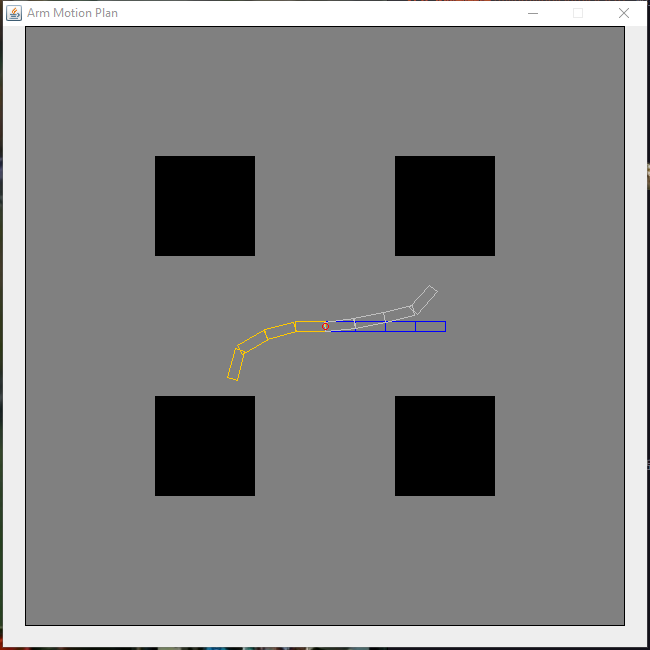
\includegraphics[width=\linewidth]{arm_1}
\end{subfigure}
\begin{subfigure}{0.4\textwidth}
  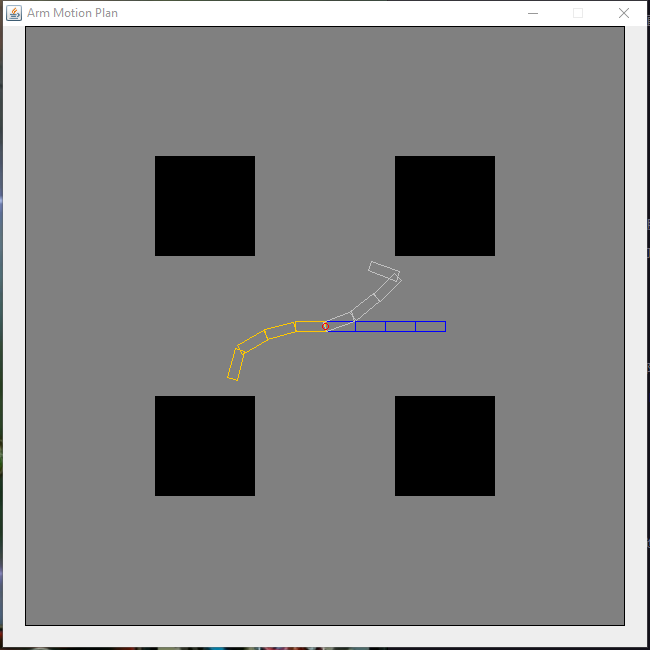
\includegraphics[width=\linewidth]{arm_2}
\end{subfigure}
\caption{Arm Motion Plan 1}
\end{figure}

\begin{figure}[!htb]
\centering
\begin{subfigure}{0.4\textwidth}
  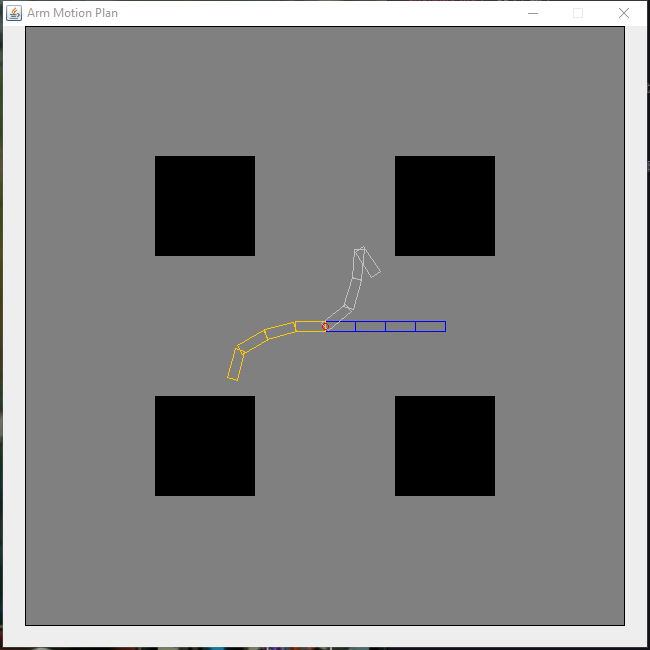
\includegraphics[width=\linewidth]{arm_3}
\end{subfigure}
\begin{subfigure}{0.4\textwidth}
  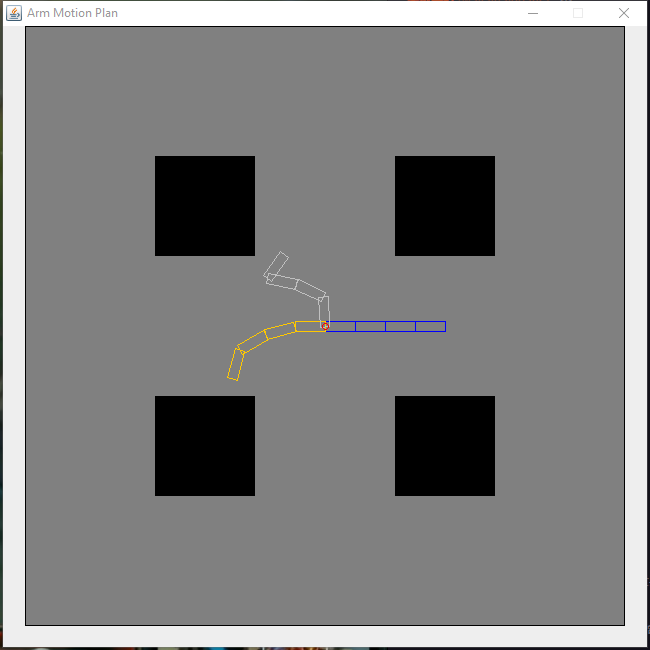
\includegraphics[width=\linewidth]{arm_4}
\end{subfigure}
\caption{Arm Motion Plan 2}
\end{figure}

\begin{figure}[!htb]
\centering
\begin{subfigure}{0.4\textwidth}
  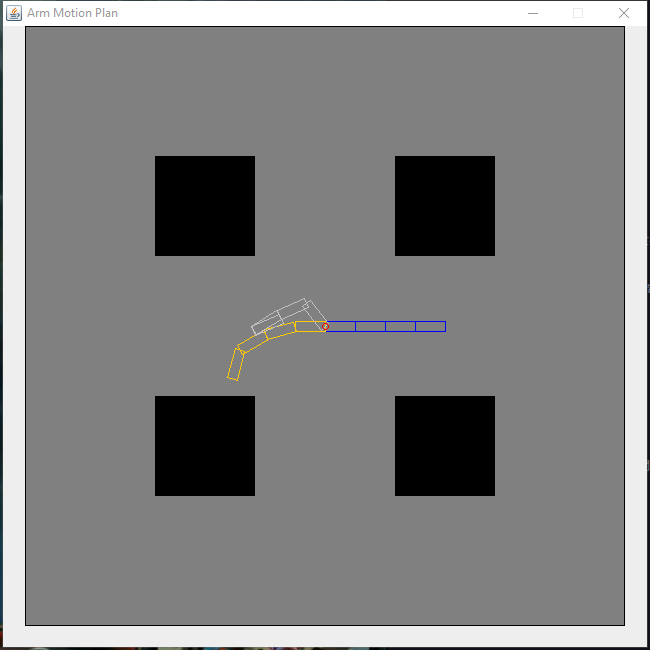
\includegraphics[width=\linewidth]{arm_5}
\end{subfigure}
\begin{subfigure}{0.4\textwidth}
  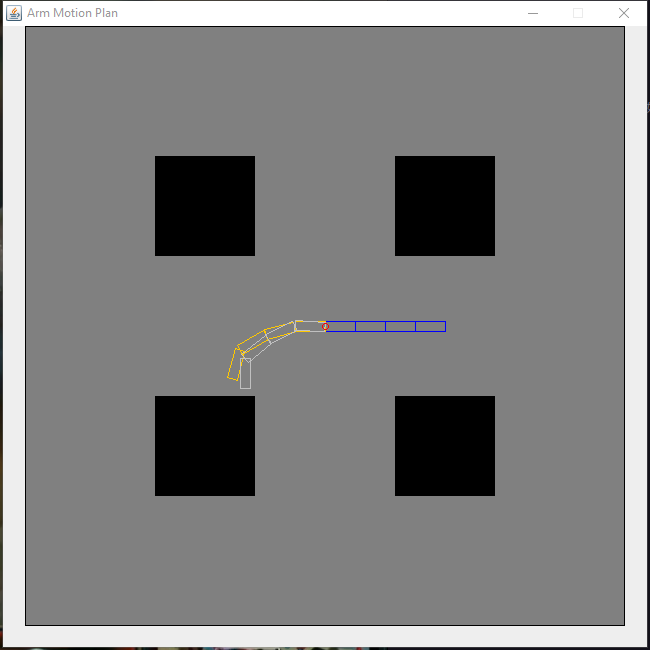
\includegraphics[width=\linewidth]{arm_6}
\end{subfigure}
\caption{Arm Motion Plan 3}
\end{figure}

\section{Rapid Exploring Random Tree}
\subsection{Basic Idea}
The basic idea of RRT is to grow a tree from the start and to fill up the configuration space. Different from the PRM method, we do not add the randomly generated node into the dataset. Rather, we use the randomly generated node as a sample to grow the tree to that direction. I think the advantage of this method is that it can generate the sample points much faster than PRM and can fill up the configuration space efficiently.

\clearpage
\subsection{Code implementation}
\subsubsection{constructor}
The constructor will get the start, goal, world, density, seed, move\_ratio and the linear velocity. Note the the linear velocity will change the moving radius of the car as I think radius = 1 is too small to show on screen.
\begin{lstlisting}
	public SteerCarProblem(World w, double[] s, double[] g, int density,
		 long seed, double move_ratio, int speed) {
		start = new double[3];
		for (int i = 0; i < 3; i++)
			start[i] = s[i];
		goal = new double[3];
		for (int i = 0; i < 3; i++)
			goal[i] = g[i];
		world = w;
		car_radius = 10;
		startNode = new SteerCarNode(start, this, -1);
		samples = new HashSet<SteerCarNode>();
		rrt = new HashMap<SteerCarNode, HashSet<SteerCarNode>>();
		samples.add((SteerCarNode) startNode);
		rrt.put((SteerCarNode) startNode, new HashSet<SteerCarNode>());
		mr = move_ratio;
		setVol(speed);
		System.out.println("Tree Constructing...");
		growTree(seed, density, move_ratio);
	}
\end{lstlisting}

\subsubsection{growTree}
The method $growTree(long, int, double) : void$ is the method to grow the tree until the number of nodes in tree reaches $density$. To grow one node from the original tree, we first generate a random node, then we find the nearest node from the tree to that random node. After that, we try to grow a node from the nearest node which is the nearest among all those options.
\begin{lstlisting}
	// Construct the tree, two methods are used:
	private void growTree(long seed, int density, double move_ratio) {
		Random rd = new Random(seed);
		while (samples.size() < density + 2) {
			// Generate a random car node
			double[] rndConfig = new double[3];
			rndConfig[0] = rd.nextDouble() * world.getWidth();
			rndConfig[1] = rd.nextDouble() * world.getHeight();
			rndConfig[2] = rd.nextDouble() * Math.PI * 2;
			SteerCarNode rndCar = new SteerCarNode(rndConfig, this, 0);
			// Expand tree if random car node is legal
			if (!rndCar.carCollide(world)) {
				SteerCarNode nearest = nearestCar(rndCar);
				SteerCarNode expandNode = expandTree(nearest, rndCar, move_ratio);
				// if no such node that can be expand, exit
				if (expandNode == null) {
					System.out.println("Expand tree failed!");
					System.exit(0);
				}
				// Expand tree if expand node is a new node
				if (!samples.contains(expandNode)) {
					samples.add(expandNode);
					rrt.get(nearest).add(expandNode);
					rrt.put(expandNode, new HashSet<SteerCarNode>());
					// if new node is close enough to the goal, break
					if (expandNode.goalTest())
						break;
				}
			}
			System.out.println(Integer.toString(samples.size()) + "/" 
				+ Integer.toString(density + 2) + " Done!");
		}

		if (samples.size() >= density + 2) {
			System.out.println("Fail to find a close enough node, 
				use the closest node as the goal, which is:");
			double dist = Double.MAX_VALUE;
			SteerCarNode goalNearest = null;
			for (SteerCarNode cur : samples) {
				if (cur.getDistance(getGoal()) < dist) {
					goalNearest = cur;
					dist = cur.getDistance(getGoal());
				}
			}
			System.out.println(goalNearest.toString());
			goal[0] = goalNearest.getState(0);
			goal[1] = goalNearest.getState(1);
			goal[2] = goalNearest.getState(2);
		}
	}
\end{lstlisting}

\subsubsection{nearestCar}
The method $nearestCar(SteerCarNode):SteerCarNode$ will return the nearest node from the tree given a random generated node. 
\begin{lstlisting}
	public List<SteerCarNode> smoothPath(List<SearchNode> path, 
		double step_size) {
		List<SteerCarNode> res = new ArrayList<SteerCarNode>();
		res.add((SteerCarNode) (path.get(0)));
		for (int i = 0; i < path.size() - 1; i++) {
			SteerCarNode curNode = (SteerCarNode) (path.get(i));
			SteerCarNode nextNode = (SteerCarNode) (path.get(i + 1));
			List<SteerCarNode> locPath = curNode.getPath(nextNode.getControl(), 
				mr, step_size);
			res.addAll(locPath);
		}
		return res;
	}
\end{lstlisting}

\subsubsection{expandTree}
The method $expandTree(SteerCarNode, SteerCarNode, double):SteerCarNode$ will return a new generated node from the tree that closest to the random generated node.
\begin{lstlisting}
	// Decide the expanding node according to a random car node,
	// by trying to expand the tree in 6 directions. This method
	// us used by method growTree(long, int): void
	private SteerCarNode expandTree(SteerCarNode nearest, 
		SteerCarNode rndCar, double move_ratio) {
		double minDis = Double.MAX_VALUE;
		SteerCarNode expandCar = null;
		for (int i = 0; i < 6; i++) {
			SteerCarNode cur = nearest.moveCar(i, move_ratio);
			if (!cur.carCollide(world) && 
				!nearest.carPathCollide(world, i, move_ratio, 0.01)) {
				double dis = cur.getDistance(rndCar);
				if (minDis > dis) {
					minDis = dis;
					expandCar = cur;
				}
			}
		}
		return expandCar;
	}
\end{lstlisting}

\subsection{Output Demonstration}
The input of the demo is as follows:
\begin{lstlisting}
		// Create the world
		world = new World(600, 600);
		world.addWall(60, 0, 540, 30);
		world.addWall(0, 275, 540, 30);
		world.addWall(60, 570, 540, 30);
		world.addObs(80, 80, 40);
		world.addObs(200, 80, 60);
		world.addObs(380, 80, 100);
		world.addObs(80, 400, 40);
		world.addWall(350, 400, 250, 40);

		// Create ArmRobot and get the path
		double[] start = { 15, 15, 0 };
		double[] goal = { 30, 570, 0 };
		carRobot = new SteerCarProblem(world, start, goal, 10000, 2016, 3, 10);
\end{lstlisting}

The result is shown as follow. The blue rectangle area is the starting point, the green rectangle area is the goal point. The blue cycle is the car. The green path is the car path and the red dot on the car point the direction of the car. The dark gray dot is the generated tree.

\begin{figure}[!htb]
\centering
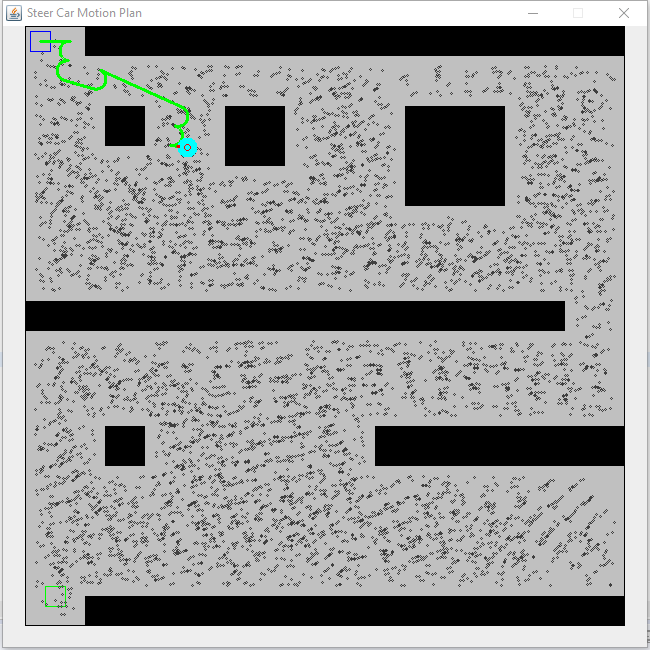
\includegraphics[width=\linewidth]{car_11}
\caption{Car Motion Plan 1}
\end{figure}
\begin{figure}[!htb]
\centering
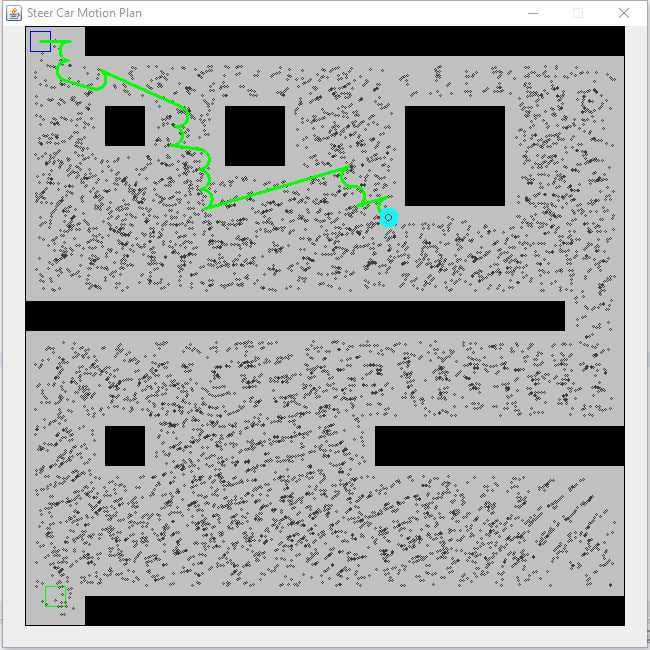
\includegraphics[width=\linewidth]{car_12}
\caption{Car Motion Plan 2}
\end{figure}
\begin{figure}[!htb]
\centering
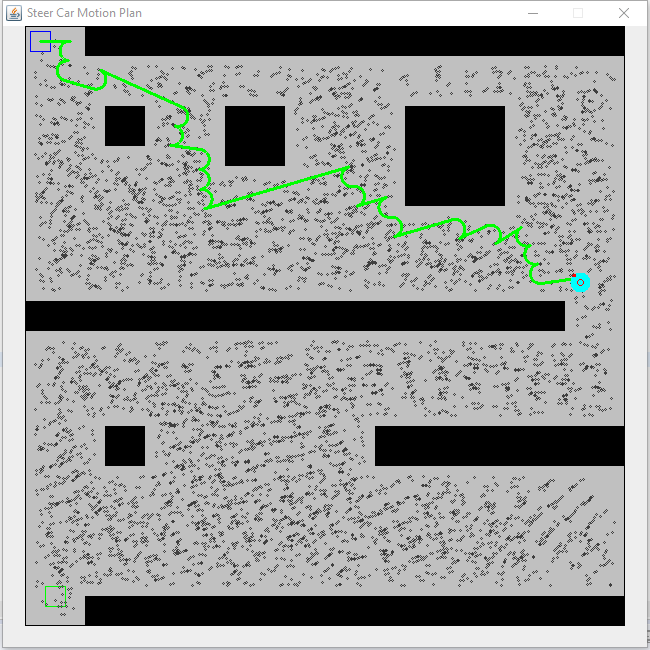
\includegraphics[width=\linewidth]{car_13}
\caption{Car Motion Plan 3}
\end{figure}
\begin{figure}[!htb]
\centering
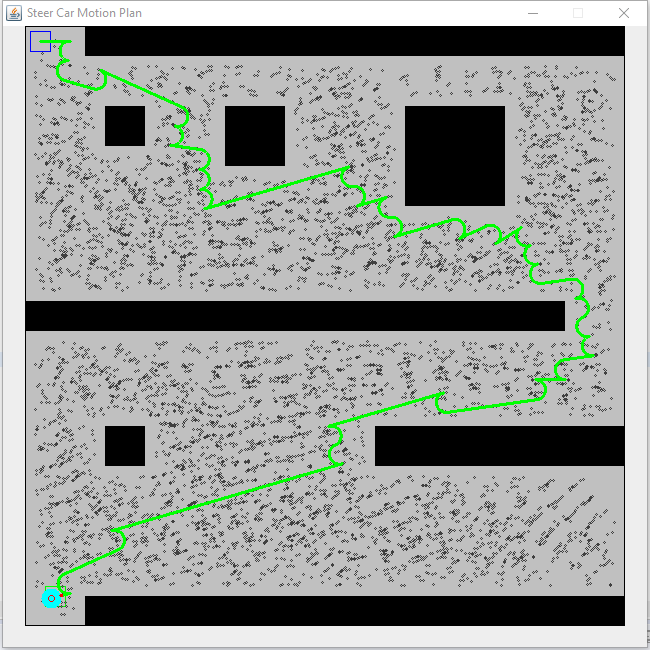
\includegraphics[width=\linewidth]{car_14}
\caption{Car Motion Plan 4}
\end{figure}

\clearpage
\section{Previous Work}
For the RRT part, I read the paper "RRT-connect: An efficient approach to single-query path planning." by Kuffner Jr, James J., and Steven M. LaValle. The paper majorly describes a method of building the RRT tree from start and goal at the same time. Interestingly I have been thinking about this method while I was doing the assignment as there was always the possibility that the program cannot grow the tree to a close enough place to the goal. To me, this is a kind of bi-direction BFS versus the normal BFS method.


For the PRM part, I read the paper "Asymptotically Near-Optimal Planning with Probabilistic Roadmap Spanners" by James D. Marble and Kostas E. Bekris. This paper introduces two methods that can reduce the construction time and density of graph while still providing a nearly same optimal result comparing to the normal PRM method. The first method is to build a roadmap spanner in a sequential manner and the second method is to interleave roadmap construction with a spanner preserving filter. By the methods introduced in this paper, the query time for the map reduces significantly and thus accelerate the process of PRM.
\end{document}